%!TEX program = xelatex
\documentclass[11pt, a4paper]{article}

% AA LINGUA E GESTIONE FONT (Specifica per XeLaTeX)
\usepackage{fontspec}
\setmainfont{Latin Modern Roman}
\usepackage[italian]{babel}

% AA LAYOUT DI PAGINA E TIPOGRAFIA (Ottimizzato per Rilegatura)
\usepackage[left=2.4cm, right=1.6cm, top=2cm, bottom=2cm]{geometry}

% AA Spaziatura tra paragrafi controllata (compatta ed evita salti enormi)
\usepackage[skip=3pt plus 1pt minus 1pt]{parskip}
\setlength{\parindent}{0pt}

% AA Microtype per XeLaTeX
\usepackage[protrusion=true]{microtype}
\raggedbottom

% AA GESTIONE DEI COLORI
\usepackage{xcolor}

% AA MATEMATICA E SIMBOLI
\usepackage{amsmath}
\usepackage{mathtools}
\usepackage{silence}
\usepackage[warnings-off={mathtools-overbracket,mathtools-colon}]{unicode-math}
\setmathfont{Latin Modern Math}

% BB OTTIMIZZAZIONE MATRICI LUNGHE PER LA STAMPA
\setlength{\arraycolsep}{10pt}

% AA Spaziature verticali attorno alle formule matematiche
\setlength{\abovedisplayskip}{3pt plus 1pt minus 1pt}
\setlength{\belowdisplayskip}{3pt plus 1pt minus 1pt}
\setlength{\abovedisplayshortskip}{0pt plus 1pt}
\setlength{\belowdisplayshortskip}{2pt plus 1pt minus 1pt}

% AA GRAFICA ED IMMAGINI
\usepackage{graphicx}
\graphicspath{{./E1_Images/}}
\usepackage{float}

% AA PERSONALIZZAZIONE TITOLI
\usepackage{titlesec}
\titleformat{\section}{\normalfont\Large\bfseries\color{blue!80!black}}{\thesection}{1em}{}
\titleformat{name=\section,numberless}{\normalfont\Large\bfseries\color{blue!80!black}}{}{0pt}{}

\titleformat{\subsection}{\normalfont\large\bfseries}{\thesubsection}{1em}{}
\titleformat{name=\subsection,numberless}{\normalfont\large\bfseries}{}{0pt}{}

\titleformat{\subsubsection}{\normalfont\normalsize\bfseries}{\thesubsubsection}{1em}{}
\titleformat{name=\subsubsection,numberless}{\normalfont\normalsize\bfseries}{}{0pt}{}

\titlespacing*{\section}{0pt}{1.2ex plus 0.4ex minus 0.2ex}{0.6ex plus 0.2ex}
\titlespacing*{\subsection}{0pt}{1ex plus 0.3ex minus 0.2ex}{0.5ex plus 0.2ex}
\titlespacing*{\subsubsection}{0pt}{0.8ex plus 0.2ex minus 0.1ex}{0.4ex plus 0.1ex}

\titleformat{\paragraph}[block]{\normalfont\normalsize\bfseries\color{black!80!black}\raggedright}{}{0pt}{}
\titlespacing*{\paragraph}{0pt}{1.2ex plus 0.3ex minus 0.2ex}{0.4ex}

% AA INTEGRAZIONE CODICE MATLAB
\usepackage{matlab}

% BB Riconfigurazione Automatica Titoli Esportati da MATLAB
\renewcommand{\matlabheading}[1]{\section*{#1}}
\renewcommand{\matlabheadingtwo}[1]{\subsection*{#1}}
\renewcommand{\matlabheadingthree}[1]{\subsubsection*{#1}}

% BB Formule E Matrici Simboliche
\renewenvironment{matlabsymbolicoutput}{%
  \par\vspace{2pt}%
  \begingroup
  \centering
}{%
  \par\vspace{2pt}%
  \endgroup
}

% BB Output Testuale Console
\renewenvironment{matlaboutput}{%
  \par\vspace{1pt}%
  \Verbatim[xleftmargin=10pt, formatcom=\color{black!75}, fontsize=\footnotesize]%
}{%
  \endVerbatim
  \vspace{1pt}%
}

% BB Box Codice (Stile Moderno con Barra Laterale Colorata)
\lstset{
  backgroundcolor={},
  aboveskip=0pt,
  belowskip=0pt,
  basicstyle=\ttfamily\footnotesize,
  xleftmargin=0pt
}

\mdfdefinestyle{matlabcode}{%
  topline=false,
  bottomline=false,
  rightline=false,
  leftline=true,
  linewidth=2.5pt,
  linecolor=blue!75!black,
  backgroundcolor=black!3,
  innertopmargin=4pt,
  innerbottommargin=4pt,
  innerleftmargin=9pt,
  innerrightmargin=6pt,
  skipabove=3pt,
  skipbelow=3pt
}

\allowdisplaybreaks

% AA LINK, METADATI ED ELENCHI
\usepackage{hyperref}
\hypersetup{
    colorlinks=true,
    linkcolor=blue!80!black,
    urlcolor=blue!80!black,
    citecolor=blue!80!black,
    pdftitle={Rappresentazione Asse-Angolo},
    pdfauthor={Francesco Lo Verde},
}
\usepackage{bookmark}

% BB Spaziatura Elenchi (Arieggiata per la Stampa)
\usepackage{enumitem}
\setlist{itemsep=3.5pt plus 1pt minus 1pt, topsep=4pt plus 1pt minus 1pt, partopsep=0pt, parsep=1pt}

\author{Francesco Lo Verde}
\begin{document}

\matlabtitle{Rappresentazione Asse-Angolo}

\begin{par}
\begin{flushleft}
La rappresentazione Asse-Angolo è un metodo per descrivere l'orientamento di un corpo rigido nello spazio. Utilizza quattro parametri:
\end{flushleft}
\end{par}

\begin{itemize}
\setlength{\itemsep}{-1ex}
   \item{\begin{flushleft} Un \textbf{versore} $\mathbf{r}=[r_X ,r_Y ,r_Z ]$ che definisce l'asse attorno al quale avviene la rotazione. \end{flushleft}}
   \item{\begin{flushleft} Un \textbf{angolo} $\theta$, che indica l'ampiezza della rotazione attorno a tale asse. \end{flushleft}}
\end{itemize}

\matlabheadingtwo{Problema Diretto}

\begin{par}
\begin{flushleft}
Il problema diretto consiste nel determinare la matrice di rotazione $R\bigl(\theta ,\mathbf{r}\bigr)$ partendo da un asse $\mathbf{r}$ e un angolo $\theta$. La matrice di rotazione si ottiene tramite la \textit{formula di Rodrigues}, derivata dalla composizione di rotazioni elementari:
\end{flushleft}
\end{par}

\begin{par}
$$R(\theta ,r)=rr^T +(I-rr^T )\cos (\theta )+S(r)\sin (\theta )$$
\end{par}

\begin{par}
\begin{flushleft}
Dove:
\end{flushleft}
\end{par}

\begin{par}
\begin{flushleft}
$I$ è la matrice identità 3x3.
\end{flushleft}
\end{par}

\begin{par}
\begin{flushleft}
$rr^T$è il prodotto esterno del versore $\mathbf{r}$
\end{flushleft}
\end{par}

\begin{par}
\begin{flushleft}
$S(r)$ è la Skew-Symmetric Matrix associata a $\mathbf{r}$, che rappresenta l'operatore prodotto vettoriale:
\end{flushleft}
\end{par}

\begin{par}
$$S(r)=\left(\begin{array}{ccc}
0 & -r_z  & r_y \\
r_z  & 0 & -r_x \\
-r_y  & r_x  & 0
\end{array}\right)$$
\end{par}

\begin{matlabcode}
clc; clear; close all;
% Definizione variabili simboliche
syms rx ry rz theta real

% Definiamo il versore r come un vettore colonna
r = [rx; ry; rz];
[R] = Compute_Rotation_Matrix(r, theta);

disp("Matrice Di Rotazione R(theta, r):");
\end{matlabcode}
\begin{matlaboutput}
Matrice Di Rotazione R(theta, r):
\end{matlaboutput}
\begin{matlabcode}
disp(R);
\end{matlabcode}
\begin{matlabsymbolicoutput}
\hskip1em $\displaystyle \begin{array}{l}
\left(\begin{array}{ccc}
{\textrm{rx}}^2 -\cos \left(\theta \right)\,{\left({\textrm{rx}}^2 -1\right)} & \textrm{rx}\,\textrm{ry}-\textrm{rz}\,\sin \left(\theta \right)-\sigma_3  & \textrm{rx}\,\textrm{rz}+\textrm{ry}\,\sin \left(\theta \right)-\sigma_2 \\
\textrm{rx}\,\textrm{ry}+\textrm{rz}\,\sin \left(\theta \right)-\sigma_3  & {\textrm{ry}}^2 -\cos \left(\theta \right)\,{\left({\textrm{ry}}^2 -1\right)} & \textrm{ry}\,\textrm{rz}-\textrm{rx}\,\sin \left(\theta \right)-\sigma_1 \\
\textrm{rx}\,\textrm{rz}-\textrm{ry}\,\sin \left(\theta \right)-\sigma_2  & \textrm{ry}\,\textrm{rz}+\textrm{rx}\,\sin \left(\theta \right)-\sigma_1  & {\textrm{rz}}^2 -\cos \left(\theta \right)\,{\left({\textrm{rz}}^2 -1\right)}
\end{array}\right)\\
\mathrm{}\\
\textrm{where}\\
\mathrm{}\\
\;\;\sigma_1 =\textrm{ry}\,\textrm{rz}\,\cos \left(\theta \right)\\
\mathrm{}\\
\;\;\sigma_2 =\textrm{rx}\,\textrm{rz}\,\cos \left(\theta \right)\\
\mathrm{}\\
\;\;\sigma_3 =\textrm{rx}\,\textrm{ry}\,\cos \left(\theta \right)
\end{array}$
\end{matlabsymbolicoutput}

\newpage
\matlabheadingthree{Calcoli Numerici Problema Diretto}

\begin{par}
\begin{flushleft}
Si calcola la matrice di rotazione numerica e successivamente si verificano le proprietà fondamentali.
\end{flushleft}
\end{par}

\begin{matlabcode}
% Definizione del vettore r e dell'angolo theta numerici
rNum = [1; 2; 3];
thetaNum = -7*pi/9;

% Verifica se il vettore r ha 3 componenti
if numel(rNum) == 3
    disp("Il Vettore r Ha 3 Componenti!");
else
    % Uso 'error' per interrompere l'esecuzione in caso di errore
    error("Il Vettore r Deve Avere 3 Componenti!");
end
\end{matlabcode}
\begin{matlaboutput}
Il Vettore r Ha 3 Componenti!
\end{matlaboutput}
\begin{matlabcode}

% Verifica se theta è uno scalare
if isscalar(thetaNum)
    disp("Theta È Uno Scalare");
else
    % Uso 'error' per interrompere l'esecuzione in caso di errore
    error("Theta Deve Essere Uno Scalare!");
end
\end{matlabcode}
\begin{matlaboutput}
Theta È Uno Scalare
\end{matlaboutput}
\begin{matlabcode}

% Si controlla che r sia un vettore colonna 3x1
rNum = reshape(rNum, [3, 1]);

% Calcolo della norma di r
norm_rNum = norm(rNum);


if norm_rNum > 0
    % Il vettore r ha una direzione ben definita (non è il vettore nullo).
    % Normalizzo il vettore r per ottenere un vettore unitario che
    % rappresenta l'asse di rotazione.

    disp("Normalizzo Il Vettore r...");
    rNum = rNum / norm_rNum;

    disp("Vettore r Normalizzato:");
    disp(rNum);
else
    % Se la norma è nulla, il vettore r è il vettore nullo.
    % Non c'è alcuna direzione valida per l'asse di rotazione.
    % Imposto theta = 0 per indicare che non c'è rotazione (R = I).
    disp("Il Vettore r È Nullo. Imposto Theta = 0.");
    thetaNum = 0;
end
\end{matlabcode}
\begin{matlaboutput}
Normalizzo Il Vettore r...
Vettore r Normalizzato:
    0.2673
    0.5345
    0.8018
\end{matlaboutput}
\newpage
\begin{matlabcode}
[R] = Compute_Rotation_Matrix(rNum, thetaNum);

disp("Matrice Di Rotazione R(theta, r) Numerica:");
disp(R);
\end{matlabcode}
\begin{matlaboutput}
Matrice Di Rotazione R(theta, r) Numerica:
\end{matlaboutput}
\begin{matlaboutput}
   -0.2155   -0.5755    0.7889
    0.9495    0.0650    0.3068
   -0.2279    0.8152    0.5325
\end{matlaboutput}

\begin{par}
\begin{flushleft}
Una matrice di rotazione \textbf{R} gode di importanti proprietà:
\end{flushleft}
\end{par}

\begin{enumerate}
\setlength{\itemsep}{1ex}
   \item{\begin{flushleft} \textbf{Ortogonalità:} La matrice è ortogonale, ovvero la sua inversa coincide con la sua trasposta $(R^T R=I)$. \end{flushleft}}
   \item{\begin{flushleft} \textbf{Determinante Unitario: }$\det (R)=1$ \end{flushleft}}
   \item{\begin{flushleft} \textbf{Traccia: }La traccia è legata all'angolo di rotazione dalla formula $\textrm{trace}(R)=1+2\cos (\theta )$. \end{flushleft}}
\end{enumerate}

\begin{matlabcode}
checkOrt = R' * R;
disp('Verifica Ortogonalità (R'' * R):');
disp(checkOrt);
\end{matlabcode}
\begin{matlaboutput}
Verifica Ortogonalità (R' * R):
    1.0000    0.0000   -0.0000
    0.0000    1.0000   -0.0000
   -0.0000   -0.0000    1.0000
\end{matlaboutput}
\begin{matlabcode}
detR = det(R);
fprintf('Determinante Di R: %f\n\n', detR);
\end{matlabcode}
\begin{matlaboutput}
Determinante Di R: 1.000000
\end{matlaboutput}
\begin{matlabcode}
traceR = trace(R);
traceSim = 1 + 2*cos(thetaNum);
fprintf('Traccia Calcolata Di R: %f\n', traceR);
fprintf('Valore Atteso (1 + 2*cos(theta)): %f\n', traceSim);
\end{matlabcode}
\begin{matlaboutput}
Traccia Calcolata Di R: 0.381966
Valore Atteso (1 + 2*cos(theta)): 0.381966
\end{matlaboutput}

\matlabheadingtwo{Problema Inverso}

\begin{par}
\begin{flushleft}
Il problema inverso consiste nel determinare l'asse \textbf{r }e l'angolo $\theta$ a partire da una matrice di rotazione \textbf{R }nota.
\end{flushleft}
\end{par}

\begin{par}
\begin{flushleft}
Dalla relazione della traccia, si può isolare l'angolo $\theta$:
\end{flushleft}
\end{par}

\begin{par}
$$\textrm{trace}(R)=1+2\cos (\theta )~~\longrightarrow ~~\theta =\arccos \left(\frac{\textrm{trace}(R)-1}{2}\right)$$
\end{par}

\begin{par}
\begin{flushleft}
Questa formula restituisce un angolo nell'intervallo $[0,\pi ]$.
\end{flushleft}
\end{par}

\begin{par}
\begin{flushleft}
Per trovare l'asse di rotazione \textbf{r}, si sfrutta la parte antisimmetrica della matrice \textbf{R:}
\end{flushleft}
\end{par}

\begin{par}
$$R-R^T =2\sin (\theta )\;\mathbf{r}$$
\end{par}

\begin{par}
\begin{flushleft}

Da questa relazione, si possono estrarre le componenti di \textbf{r}
\end{flushleft}
\end{par}

\begin{par}
$$r=\frac{1}{2\sin (\theta )}\;R-R^T =\frac{1}{2\sin (\theta )}\;\left(\begin{array}{c}
r_{32} -r_{23} \\
r_{13} -r_{31} \\
r_{21} -r_{12}
\end{array}\right)$$
\end{par}

\begin{par}
\begin{flushleft}
Questo metodo è valido solo se $\sin (\theta )\not= 0$, ovvero per angoli di rotazione diversi da 0 e $k\pi$
\end{flushleft}
\end{par}
\newpage
\begin{matlabcode}
% Calcolo dell'angolo theta dalla traccia
cosTheta = (trace(R) - 1) / 2;
thetaCalc = acos(cosTheta);

% Calcolo dell'asse r
rCalc = [NaN; NaN; NaN];
sinTheta = sin(thetaCalc);

if abs(sinTheta) < 1e-9
    disp('Theta È 0 o pi. Asse Non È Definito Univocamente Con Questa Formula.');
else
    % Si estraggono le componenti dalla parte antisimmetrica di R
    rVec = [R(3,2) - R(2,3); R(1,3) - R(3,1); R(2,1) - R(1,2)];
    rCalc = (1 / (2 * sinTheta)) * rVec;
end

disp('Valori Input:');
fprintf('Theta = %.4f rad\n', thetaNum);
disp('Vettore r =');
disp(rNum);
\end{matlabcode}
\begin{matlaboutput}
Valori Input:
Theta = 1.8850 rad
Vettore r =
    0.2673
    0.5345
    0.8018
\end{matlaboutput}

\begin{matlabcode}
disp('Valori Calcolati Dal Problema Inverso:');
fprintf('Theta Calcolato = %.4f rad\n', thetaCalc);
disp('Vettore r Calcolato =');
disp(rCalc);
\end{matlabcode}
\begin{matlaboutput}
Valori Calcolati Dal Problema Inverso:
Theta Calcolato = 1.8850 rad
Vettore r Calcolato =
    0.2673
    0.5345
    0.8018
\end{matlaboutput}
\begin{matlabcode}
% Calcolo dell'errore per verificare la correttezza
fprintf('Errore Su Theta: %e\n', abs(thetaNum - thetaCalc));
fprintf('Errore Su r: %e\n', norm(rNum - rCalc));
\end{matlabcode}
\begin{matlaboutput}
Errore Su Theta: 0.000000e+00
Errore Su r: 0.000000e+00
\end{matlaboutput}
\newpage
\matlabheadingtwo{Visualizzazione Grafica}

\begin{matlabcode}
% Assi Sistema Riferimento
AsseX = [1, 0, 0];
AsseY = [0, 1, 0];
AsseZ = [0, 0, 1];

% Vettore Da Ruotare
v = [1; 0; 1];

% Calcolo Vettore Ruotato
vR = R * v;

% Impostazioni Figura
figure;
hold on;
grid off;
box off;
axis off;
rotate3d on;

% Disegno Assi Cartesiani
quiver3(0, 0, 0, AsseX(1), AsseX(2), AsseX(3), 'r', 'LineWidth', 2, 'DisplayName', 'Asse X');
quiver3(0, 0, 0, AsseY(1), AsseY(2), AsseY(3), 'g', 'LineWidth', 2, 'DisplayName', 'Asse Y');
quiver3(0, 0, 0, AsseZ(1), AsseZ(2), AsseZ(3), 'b', 'LineWidth', 2, 'DisplayName', 'Asse Z');

% Etichette Assi
text(AsseX(1), AsseX(2), AsseX(3), ' X', 'FontSize', 10, 'Color', 'r', 'FontWeight', 'bold');
text(AsseY(1), AsseY(2), AsseY(3), ' Y', 'FontSize', 10, 'Color', 'g', 'FontWeight', 'bold');
text(AsseZ(1), AsseZ(2), AsseZ(3), ' Z', 'FontSize', 10, 'Color', 'b', 'FontWeight', 'bold');

% Disegno Asse Rotazione
plot3([0, rNum(1)], [0, rNum(2)], [0, rNum(3)], '--', 'Color', [0, 0.5, 0.5], 'LineWidth', 2, 'DisplayName', 'Asse Rotazione r');
text(rNum(1), rNum(2), rNum(3), ' Asse r', 'Color', [0, 0.5, 0.5], 'FontSize', 11, 'FontWeight', 'bold');

% Disegno Vettore Iniziale
quiver3(0, 0, 0, v(1), v(2), v(3), 0, 'k', 'LineWidth', 1.5, 'DisplayName', 'Vettore v');
text(v(1), v(2), v(3), ' v', 'FontSize', 11, 'Color', 'k');

% Disegno Vettore Ruotato
quiver3(0, 0, 0, vR(1), vR(2), vR(3), 0, 'm', 'LineStyle', ':', 'LineWidth', 2.5, 'DisplayName', 'Vettore R*v');
text(vR(1), vR(2), vR(3), ' R*v', 'FontSize', 11, 'Color', 'm');

% Titolo della figura
title(['Rotazione di ', num2str(rad2deg(thetaNum), '%.1f'), ' gradi Attorno a r']);

axis equal;
view(50, 20);

hold off;
\end{matlabcode}
\begin{center}
% \includegraphics[width=\maxwidth{32.5137982940291em}]{figure_0.png}
\begin{figure}[H]
    \centering
    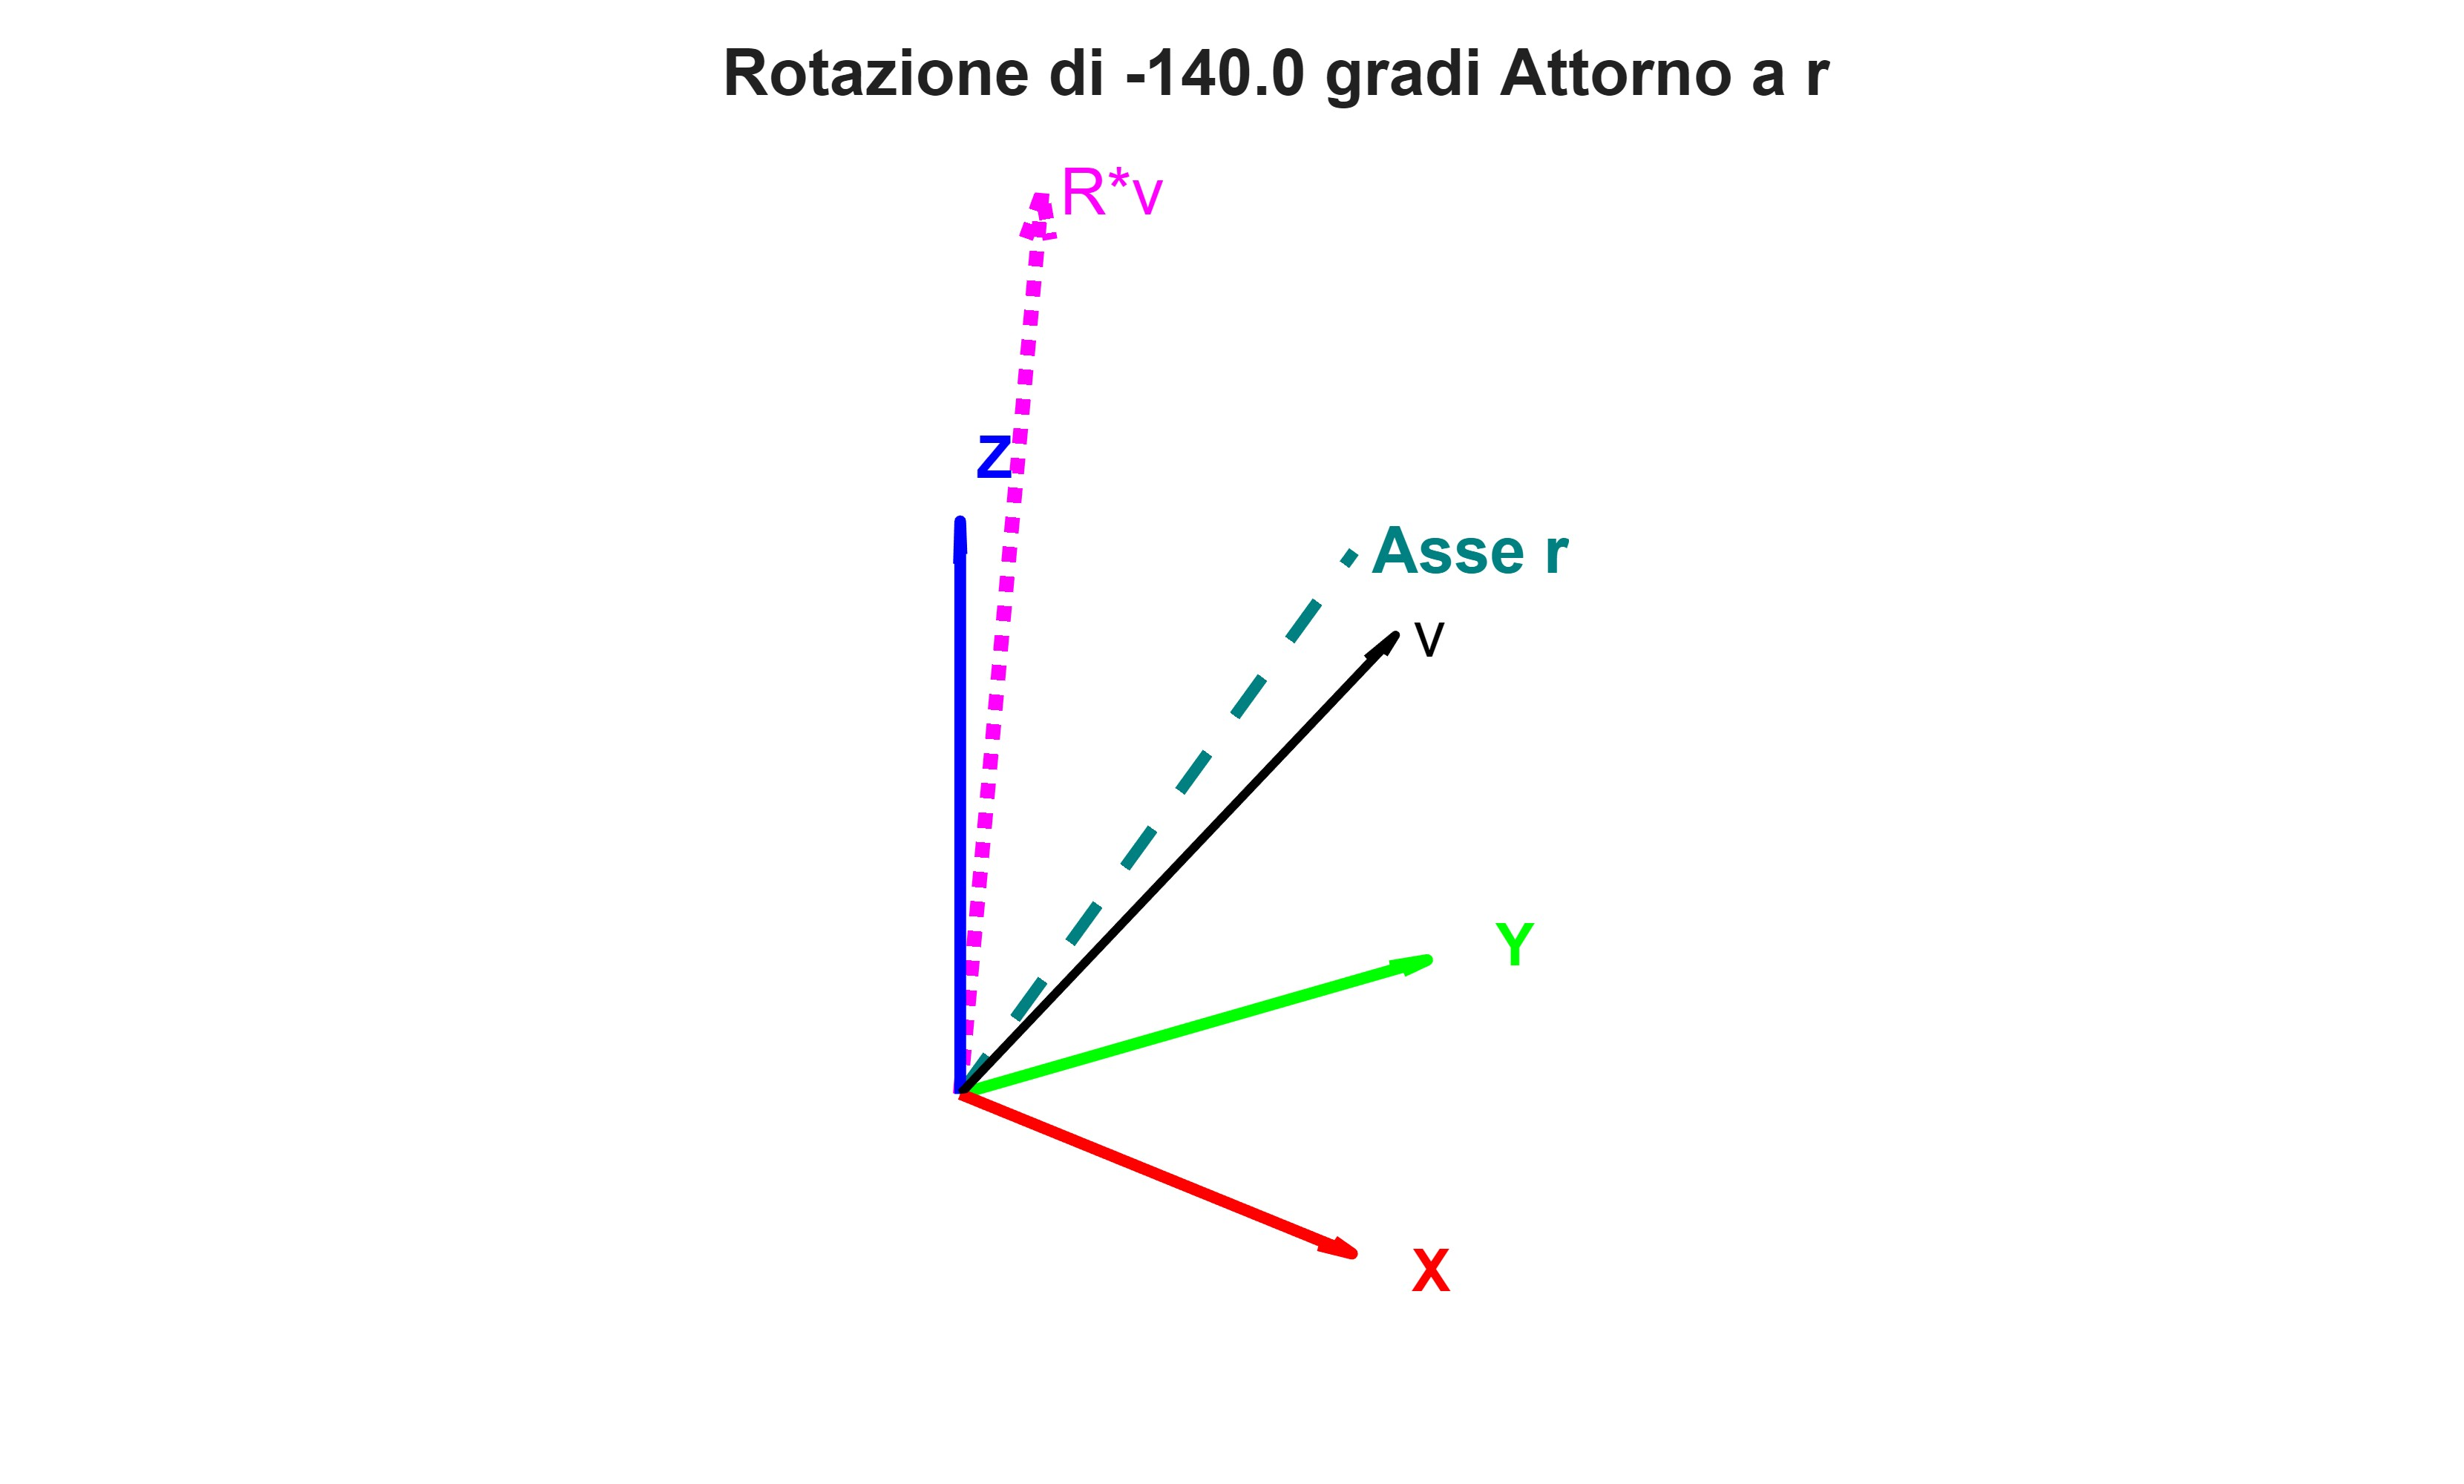
\includegraphics[width=0.99\linewidth]{figure_0.jpeg}
\end{figure}
\end{center}

\end{document}
